\section{Graphabdeckung}
\label{graphueberdeckung}

Wie zuvor gesehen, existieren verschiedene Abdeckungskriterien um Testabdeckung zu prüfen.
Die Graphabdeckung führt verschiedene Kriterien ein, die es ermöglichen, aus Graphen Pfade für Tests zu generieren.
GraphQL kann, wie in Kapitel~\ref{graphtheorieQL} gesehen, durch einen Graphen repräsentiert werden.
Hinter jedem Knoten in diesem Graphen steckt ein Resolver der potenziell einem eigenen Modul angehört.
Anfragen an GraphQL können nun Resolver beliebig miteinander kombinieren.
Um diese Kombinationen zu testen, wollen wir Graphabdeckungskriterien nutzen, um Tests zu generieren,
die für eine ausreichende Testabdeckung zu sorgen.
Da in GraphQL zyklische Graphen erlaubt sind, ist der Testraum potentiell unendlich groß.
Dieses Problem kann durch die Verwendung von Graphabdeckung gelöst werden.
Zuerst müssen wir ersteinmal weitere Theorie einführen.
Um Graphcoverage zu nutzen, verfeinern wir die allgemeine Definition~\ref{gerichtetergraphdef} von gerichteten Graphen.
Im Testkontext definieren wir einen gerichteten Graphen wie folgt:

\begin{definition}
    Ein gerichteter Graph G ist definiert als
    \begin{description}
        \item[Menge N] von Knoten
        \item[Menge N_{0}] von Anfangsknoten, wobei N_{0} $\subseteq$ N
        \item[Menge N_{f}] von Endknoten, wobei N_{f} $\subseteq$ N
        \item[Menge E] von Kanten, wobei E $\subseteq$ N x N. Hierbei ist die Menge als init{x} x target{y} definiert.
    \end{description}~\cite[2.1 Overview]{software-testing}
\end{definition}

Mithilfe dieser Definition können nun zum Beispiel Kontrollflussgraphen abgebildet werden, indem die Einstiegspunkte die Anfangsknoten sind und die Endknoten die Austrittspunkte.
Ein Pfad innerhalb von eben definierten Graphen der in einem Knoten $x \in N_{0}$ startet und in einem Knoten $y \in N_{f}$ endet, nennt sich Testpfad~\cite[vgl. Def 2.31]{software-testing}
Ziel ist es nun mithilfe von Abdeckungskriterien Testpfade zu ermitteln die einen Graphen ausreichend abdecken.
Ein Graph gilt als ausreichend abgedeckt wenn die folgende Definition~\ref{graphcov} gilt.

\begin{definition}
    Gegeben sei eine Menge $TR$ von Testanforderungen für ein Graphabdeckungskriterium $C$.
    Eine Menge Tests $T$ erfüllt $C$ auf Graphen $G$ wenn gilt: Jedes Element von $TR$ ist durch mindestens einen Pfad p abgedeckt.
    \cite[vgl. Def. 2.32]{software-testing}
    \label{graphcov}
\end{definition}

Hierfür existieren verschiedene Kriterien die wir im folgenden definieren wollen.

\subsection{Graphabdeckungskriterien}

Im folgenden Stellen wir verschiedene Graphabdeckunskriterien vor so wie sie in~\cite{software-testing} definiert werden.
Dabei ist ein Graphabdeckungskriterium eine Sammlung von Testanforderungen gemäß Definition~\ref{tr} auf Graphstrukturen.
Später folgt ein Vergleich der einzelnen Kriterien um diese besser einordnen zu können.

\subsubsection{Knotenabdeckung}

Erwartet man, dass beim Testen jede definierte Methode zumindest einmal ausgeführt wird, so handelt es sich hierbei um Knotenabdeckung.
Diese Kriterium ist weithin geläufig als $Blockabdeckung$ \cite[vgl. 2.2.1]{software-testing}.
Eine Menge $T$ an Tests erfüllt die Knotenabdeckung wenn gilt, dass jeder erreichbare Knoten durch zumindest einen Test $t \in T$ besucht wird.
Formal definieren wir dies in Definiton~\ref{nodecov}: 

\begin{definition}
    \textbf{Knotenabdeckung}: $TR$ enthält jeden erreichbaren Knoten in $G$~\cite[vgl. Criterion 2.1]{software-testing}.
    \label{nodecov}
\end{definition}


\subsubsection{Kantenabdeckung}

Eine Granularitätsebene höher ist die Kantenabdeckung.
In diesem Kriterium wird gefordert, dass jede erreichbare Kante mindestens einmal in einer gegebenen Menge an Test besucht wird.

\begin{definition}
    \textbf{Kantenabdeckung}: $TR$ enthält jeden erreichbaren Pfad der Länge bis zu 1 (Kanten), in $G$~\cite[vgl. Criterion 2.2]{software-testing}.
    \label{edgecov}
\end{definition}

Dadurch ist eingeschlossen, dass auch jeder Knoten besucht wird.
Man kann sagen, dass die Kantenabdeckung ein stärkeres Kriterium ist, da dieses die Knotenabdeckung automatisch beinhaltet.
Diese Gegebenheit wird sich weiterhin fortführen, sodass die Kriterien im generellen stärker, aber auch schwerer zu berechnen, werden.

\subsubsection{Kanten-Paar Abdeckung}

Die Kantenabdeckung betrachtet nur die einzelnen Pfade des Graphens.
Im Testkontext ist aber durchaus die zuvor ausgeführte Operation auch wichtig und muss im Testprozess berücksichtigt werden.
Um dem Rechnung zu tragen führen wir die Kanten-Paar Abdeckung ein.
Diese setzt vorraus, dass eine Menge an Tests $T$ alle möglichen Kantenpaare durch mindestens einen Test abgedeckt hat.

\begin{definition}
    \textbf{Kanten-Paar Abdeckung}: $TR$ enthält jeden erreichbaren Pfad der Länge bis zu 2 (Kanten), in $G$~\cite[vgl. Criterion 2.3]{software-testing}.
    \label{edgepaircov}
\end{definition}

\subsubsection{PrimePfad Abdeckung:}

Während die zuvor definierten Kriterien darauf achten, dass Knoten und Kanten(-paare) abgedeckt werden, müssen wir im folgenden auch in Beachtung
ziehen, dass im Testkontext durchaus alle Pfadkombinationen die existieren relevante Testfälle darstellen können.
Die Anzahl an allen azyklischen Pfadkombinationen wird jedoch selbst bei kleinen Programmen sehr schnell groß\cite[vgl. S. 35]{software-testing}.
Gleichzeitig sind viele Pfadkombinationen Teile von längeren Pfaden und somit uninteressant im Testkontext \cite[vgl. S. 35]{software-testing}.
Um dieses Problem zu lösen wird die PrimePfad Abdeckung eingeführt.

\begin{definition}
    \textbf{PrimePfad Abdeckung}: $TR$ enthält alle PrimePfade in $G$~\cite[vgl. Criterion 2.4]{software-testing}.
    \label{primecov}
\end{definition}

und ein PrimePfad ist definiert als:

\begin{definition}
    Ein Pfad von $n_{l}$ zu $n_{i}$ ist ein PrimePfad wenn gilt, dass dieser keinen Knoten doppelt enthält (mit ausnahme von Start und Endknoten) und
    der Pfad nicht Teilpfad eines anderen Pfades ist.
\end{definition}

Es sollen also die längsten, einfachen Pfade im Graphen abgedeckt werden.
So wird eine umfassendere Abdeckung als in den vorherigen Abdeckungskriterien gewährleistet da auch längere Pfadkombinationen dabei berücksichtigt werden.

\subsubsection{Vollständige Pfadabdeckung}

Idealerweise sollten Tests die gesamte Software abdecken.
Wie jedoch in Kapitel~\ref{abdeck} schon gezeigt ist dies oft nicht möglich.
Insbesondere wenn der Graph zyklisch ist, ist der Pfadraum unendlich und kann somit nicht erfüllt werden \cite[vgl. S. 36 ]{software-testing}.
Der Vollständigkeit halber wollen wir dieses Kriterium dennoch hier definieren.

\begin{definition}
    \textbf{Vollständige Pfadabdeckung}: $TR$ enthält alle Pfade in $G$~\cite[vgl. Criterion 2.7]{software-testing}.
    \label{completecov}
\end{definition}

\subsection{Vergleich der Kriterien}

















\subsection{Node Coverage}

Node-Coverage ist ein Coveragekriterium, dass alle Knoten, die von $N_{0}$ erreichbar sind, in einem Graphen abdecken soll.
Definieren wir folgenden, sehr einfachen Graphen:

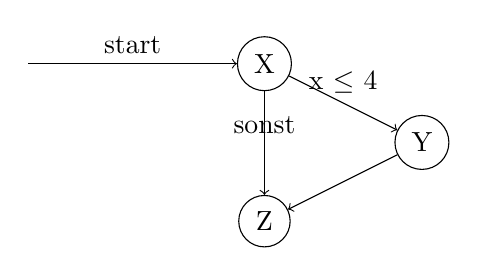
\begin{tikzpicture}
    \node[circle, draw] (n1) at (2,2) {X};
    \node[circle, draw] (n2) at (4,1) {Y};
    \node[circle, draw] (n3) at (2,0) {Z};

    \draw[->] (-1,2) -- node[above] {start} (n1);
    \draw[->] (n1) -- node[above] {x $\le$ 4} (n2);
    \draw[->] (n2) -- (n3);
    \draw[->] (n1) -- node[above] {sonst} (n3);
\end{tikzpicture}

So wäre die Node-Coverage mit einem Test einzigen Test erfüllbar.
Dieser ist der Pfad $X \rightarrow Y \rightarrow Z$.
Es ist auch denkbar, dass wir zwei Pfade oder mehr nutzen allerdings erfüllt dieser Pfad schon unser Kriterium daher geben wir uns vorerst zufrieden.
Wir sehen schnell, dass dieser Ansatz noch Lücken aufweist, da der Pfad $X \rightarrow Y \rightarrow Z$ das Kriterium erfüllt, allerdings wird eine Kante $X \rightarrow Z$ nicht im
Test berücksichtigt und kann somit ungetestet bleiben.
Wir führen also noch andere Kriterien ein, die eher geeignet wären.

\subsection{Edge-Coverage}

Edge-Coverage ist ein Coveragekriterium, dass die Kanten in einem Graphen abdecken soll.
Ziel der Edge-Coverage ist es, dass jede Kante des Graphens durch mindestens einen Test abgedeckt wird.
Um die Edge-Coverage für vorheriges Beispiel zu erreichen, benötigen wir schon zwei Routen.
Der Graph:

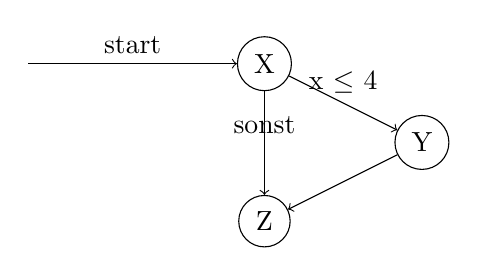
\begin{tikzpicture}
    \node[circle, draw] (n1) at (2,2) {X};
    \node[circle, draw] (n2) at (4,1) {Y};
    \node[circle, draw] (n3) at (2,0) {Z};

    \draw[->] (-1,2) -- node[above] {start} (n1);
    \draw[->] (n1) -- node[above] {x $\le$ 4} (n2);
    \draw[->] (n2) -- (n3);
    \draw[->] (n1) -- node[above] {sonst} (n3);
\end{tikzpicture}

wird über die Pfade $X \rightarrow Y \rightarrow Z$ und $X \rightarrow Z$ überdeckt.
Edge-Coverage hat allerdings auch Probleme Graphen vollständig zu überdecken.
Man nehme folgendes Beispiel:

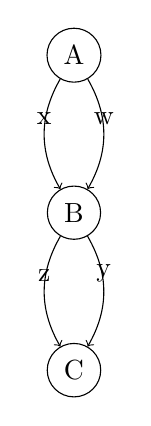
\begin{tikzpicture}
    \node[circle, draw] (a) at (4,4) {A};
    \node[circle, draw] (b) at (4,2) {B};
    \node[circle, draw] (c) at (4,0) {C};

    \draw[->, bend left=30] (a) to node[above] { w } (b);
    \draw[->, bend right=30] (a) to node[above] { x } (b);
    \draw[->, bend left=30] (b) to node[above] { y } (c);
    \draw[->, bend right=30] (b) to node[above] { z } (c);
\end{tikzpicture}

Pfade die laut Edge-Coverage ausreichen um den Graphen zu überdecken wären: \\
$ x \rightarrow z $ \\
$ w \rightarrow y $ \\
Hierbei wird allerdings außer acht gelassen, dass in $x$ auch Änderungen passieren können die Auswirkungen im Programm haben können.
So sind die Routen $ x \rightarrow y $ und $ w \rightarrow z $ in der Edge-Coverage nicht berücksichtigt.
Allerdings wären diese auch zu testen.
Wir sehen also, dass wir immer noch kein ideales Kriterium gefunden haben.


\subsection{Edge-Pair Coverage}

Das Edge-Pair Coveragekriterium ist eine Erweiterung der Edge-Coverage, indem hier auch die Beziehungen von einzelnen Kanten untereinander berücksichtigt werden um das zuvor
aufgetretene Problem zu lösen.
Nach \cite[Introduction to Software Testing]{software-testing} ist Edge-Pair Coverage: ''Alle erreichbaren Pfade von Länge bis zu 2 im Testgraphen''.
Ziel dieses Coverage-Kriteriums ist es, dass alle möglichen Kantenpaare abgedeckt sind.
Eben definiertes Beispiel hätte mit Edge-Pair Coverage eine Überdeckung mit: \\
$ x \rightarrow z $ \\
$ w \rightarrow y $ \\
$ x \rightarrow y $ \\
$ w \rightarrow z $

Dieses simple Beispiel wird durch Edge-Pair Coverage gut abgedeckt.
Edge-Pair Coverage neigt allerdings dazu, extrem große Suchräume zu erzeugen und nur Pfadkombinationen bestimmter Länge zu betrachten. \cite[vgl. S. 35]{software-testing}
Hierdurch werden bestimmte Kombinationen von Pfaden immer noch nicht berücksichtigt.

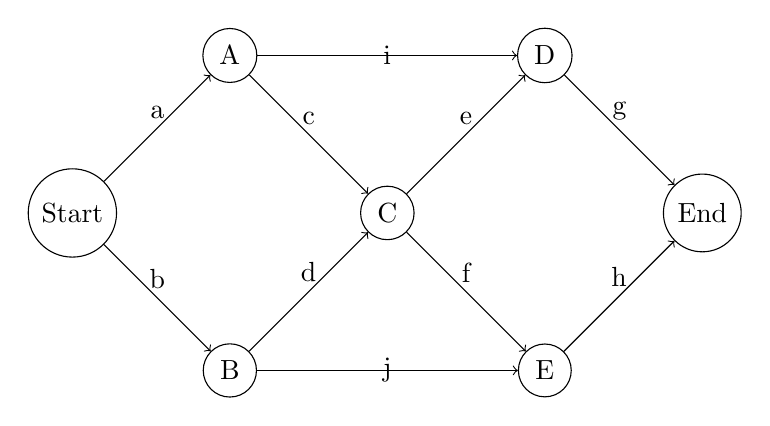
\begin{tikzpicture}
    \node[circle, draw] (start) at (0,0) {Start};
    \node[circle, draw] (a) at (2,2) {A};
    \node[circle, draw] (b) at (2,-2) {B};
    \node[circle, draw] (c) at (4,0) {C};
    \node[circle, draw] (d) at (6,2) {D};
    \node[circle, draw] (e) at (6,-2) {E};
    \node[circle, draw] (end) at (8,0) {End};

    \draw[->] (start) to node[above] { a } (a);
    \draw[->] (start) to node[above] { b } (b);
    \draw[->] (a) to node[above] { c } (c);
    \draw[->] (b) to node[above] { d } (c);
    \draw[->] (c) to node[above] { e } (d);
    \draw[->] (c) to node[above] { f } (e);
    \draw[->] (d) to node[above] { g } (end);
    \draw[->] (e) to node[above] { h } (end);
    \draw[->] (a) to node[out=30, in=150] { i } (d);
    \draw[->] (b) to node[out=-30, in=210] { j } (e);
\end{tikzpicture}

Nach der Definition von Edge-Pair Coverage ermitteln wir erstmal alle Pfadkombinationen der Länge ''bis zu 2''
Dies wären:

$Start \rightarrow A \rightarrow C$ \\
$Start \rightarrow A \rightarrow D$ \\
$Start \rightarrow B \rightarrow C$ \\
$Start \rightarrow B \rightarrow E$ \\
$A \rightarrow C \rightarrow D$ \\
$A \rightarrow C \rightarrow E$ \\
$B \rightarrow C \rightarrow D$ \\
$B \rightarrow C \rightarrow E$ \\
$A \rightarrow D \rightarrow End$ \\
$B \rightarrow E \rightarrow End$ \\
$C \rightarrow D \rightarrow End$ \\
$C \rightarrow E \rightarrow End$ \\

Hierdurch ergeben sich dann diese Testpfade:

$Start \rightarrow  A \rightarrow  C \rightarrow  D \rightarrow  End$ \\
$Start \rightarrow  A \rightarrow  C \rightarrow  E \rightarrow  End$ \\
$Start \rightarrow  B \rightarrow  C \rightarrow  D \rightarrow  End$ \\
$Start \rightarrow  B \rightarrow  C \rightarrow  E \rightarrow  End$ \\

allerdings fehlen auch hier wieder Pfade. \\
Zum Beispiel der Pfad $Start \rightarrow A \rightarrow D \rightarrow End$ fehlt.
Hierdurch bleiben wieder Teile des Graphens unüberdeckt.

\subsection{Prime-Path Coverage}

Die Prime-Path Coverage verlangt, dass jeder (Prime)Primärpfad durch mindestens einen Testpfad abgedeckt sein muss.
Ein Primärpfad ist definiert als ein einfacher Pfad, der nicht vollständig als zusammenhängender Teil in einem anderen einfachen Pfad enthalten ist. \cite[vgl. S. 35]{software-testing}
Hierbei ist ein einfacher Pfad dann  ein Pfad, in dem keine Kanten und keine Knoten wiederholt werden,
mit Ausnahme möglicherweise des ersten und letzten Knotens (wenn sie gleich sind, handelt es sich um einen Kreis).
In diesem Graphen:

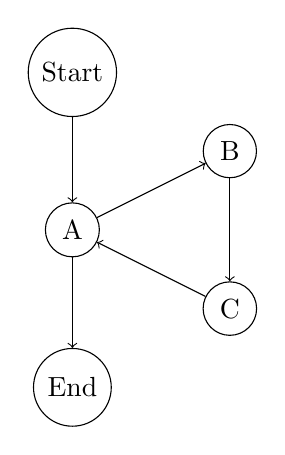
\begin{tikzpicture}
    \node[circle, draw] (start) at (4,4) {Start};
    \node[circle, draw] (a) at (4,2) {A};
    \node[circle, draw] (b) at (6,3) {B};
    \node[circle, draw] (c) at (6,1) {C};
    \node[circle, draw] (d) at (4,0) {End};


    \draw[->] (start) to node[above] { } (a);
    \draw[->] (a) to node[above] { } (b);
    \draw[->] (b) to node[above] { } (c);
    \draw[->] (a) to node[above] { } (d);
    \draw[->] (c) to node[above] { } (a);
\end{tikzpicture}

Sind dies alle Prime-Paths: \\

$ Start \rightarrow  A \rightarrow  End$ \\
$ Start \rightarrow A \rightarrow B \rightarrow C$ \\
$ A \rightarrow B \rightarrow C \rightarrow A $ \\
$ B \rightarrow C \rightarrow A \rightarrow B $ \\
$ C \rightarrow A \rightarrow B \rightarrow C $ \\
$ B \rightarrow C \rightarrow A \rightarrow End $ \\

und schon zwei Testpfade würden ausreichen um die Prime-Path Coverage zu erfüllen.
Die Testpfade die das Testrequirement erfüllen sind:

$Start \rightarrow A \rightarrow End$ \\
$Start \rightarrow A \rightarrow B \rightarrow C \rightarrow A \rightarrow B \rightarrow C \rightarrow A \rightarrow End$

\subsection{Complete-Path Coverage}

Als letztes Coveragekriterium wollen wir die Complete-Path Coverage einführen.
Ziel dieses Coveragekriteriums ist es, dass jeder mögliche Pfad mit einem Test abgedeckt werden kann.
Wir brauchen dieses Kriterium nicht ausführlich definieren, da in zyklischen Graphen eine Complete-Coverage nicht möglich ist.
Kreise in Graphen führen zu einer unendlich großen Menge an Pfaden und wir können keine unendlich große Menge behandeln.
Die Complete-Path Coverage ist sinnvoll wenn wir Kreise verbieten und der Testgraph nicht zu groß ist.
Um unsere Methode jedoch von \cite[Property-based Testing]{property-based-testing} abzugrenzen wollen wir explizit Kreise erlauben.
Ja sogar fördern um zu symbolisieren warum unsere Methode eine Verbesserung darstellt.

\subsection{abschließender Vergleich der Coverage-Kriterien}

Wir haben nun verschiedene Coverage-Kriterien kennengelernt und teilweise schon Probleme benannt die einzelne
Kriterien haben.
Im Sinne einer zufriedenstellenden Testung eines Systems wollen wir nun die einzelnen Kriterien noch einmal
zentral gegenüber stellen und sehen, welche Kriterien sich eignen würden für unseren, zu entwickelnden Prototypen.
Unser Vergleich wird 4 verschiedene Kriterien beachten, diese sind Granularität, Redundanz, Abdeckungspotential und Komplexität beziehungsweise Effizienz.
Obwohl alle Überdeckungskriterien einen einzigartigen Blick auf den Graphen bieten, so lässt sich feststellen, dass
einige Überdeckungskriterien geeigneter sind als andere.

\begin{description}
    \item[Granularität] Dieses Kriterium setzt seinen Fokus darauf, welche Teile des Graphens im Überdeckungskriterium Anwendung finden.
    Hierbei schauen wir insbesondere darauf, wie die Struktur des Graphens überdeckt wird.

    \item[Redundanz] Damit wir nicht immer wieder die selben Tests ausführen vergleichen wir, wie stark die Redundanz innerhalb
    des Überdeckungskriteriums ist. Wir wollen möglichst effizient testen da der Testprozess bei großen Systemen
    durchaus einige Zeit in Anspruch nehmen kann.
    \item[Abdeckungspotential] Wir untersuchen hier, wie stark das Potential des Kriteriums ist Tests zu generieren, die verlässlich Fehler finden.
    Hierbei ist vor allem wichtig, wie die Pfade strukturell aufgebaut sein werden die das Überdeckungskriterium erfüllen.

    \item[Komplexität / Effizienz] Mit der Komplexität und Effizienz wird untersucht, wie viele Pfade generiert werden und wie gut der mögliche Testraum durch diese
    abgebildet werden kann.
\end{description}

\newcolumntype{C}{>{\Centering\arraybackslash}X}
\begin{center}
    \begin{table}[!ht]
        \begin{tabularx}{\textwidth}{|c|c|c|c|c|}
            \hline
            \textbf{Kriterium} & \textbf{Granularität} & \textbf{Redundanz} & \textbf{Abdeckungstiefe} & \textbf{Komplexität, Effizienz}\\
            \hline
            \textbf{Node} & Knoten & Keine & Oberflächlich & Niedrigste, schnellste\\
            \hline
            \textbf{Edge} & Kanten & Minimal & Ein bisschen tiefer & Mittlere, effizient\\
            \hline
            \textbf{Edge-Pair} & Kantenpaare & Überlappung & Tiefer & Erhöhte, effizient\\
            \hline
            \textbf{SimplePath} & Pfade ohne Wiederholungen & Keine & Ziemlich tief & Hohe, langsam\\
            \hline
            \textbf{PrimePath} & Hauptpfade & Kann enthalten & Tief & Sehr hoch, langsam\\
            \hline
            \textbf{CompletePath} & Alle möglichen Pfade & Höchste & Am tiefsten & Extrem hoch, sehr langsam\\
            \hline
        \end{tabularx}
        \caption{Vergleich der Graphabdeckungskriterien}
    \end{table}
\end{center}

\section{Graphcoverage für Code}

Im Kontext der Testentwicklung erlaubt die Graphcoverage es uns, einen systematischen Ansatz zur Testgenerierung zu verfolgen.
Beziehen wir die Graphcoverage auf die Generierung von Tests für Code so müssen wir uns zuerst fragen, wie wir Code
als Graphen darstellen können.
Da dieser Abschnitt eher der generellen Einordnung dient, werden wir uns an dieser Stelle kurz halten.
Im Allgemeinen muss der Code zuerst in einen Kontrollflussgraphen überführt werden. (Quelle)
Ein Kontrollflussgraph ist ein gerichteter Graph mit, wie in 4.1 auch definiert, einer Menge Knoten, Anfangskonten und Endknoten sowie Kanten.
Wer mehr über die Umwandlung von Code in Kontrollflussgraphen lernen will, sei an \cite[Kapitel 2.]{software-testing} verwiesen.


\begin{minipage}{.5\linewidth}
    \begin{lstlisting}
function example(x, y) {
    if (x > 10) {
        if(x > 100){
            return x;
        }
        example(x - 5, y);
    } else {
        if (y < 5) {
            return y;
        }
        return x;
    }
}
    \end{lstlisting}

\end{minipage}%
\begin{minipage}{.5\linewidth}
    \begin{center}
        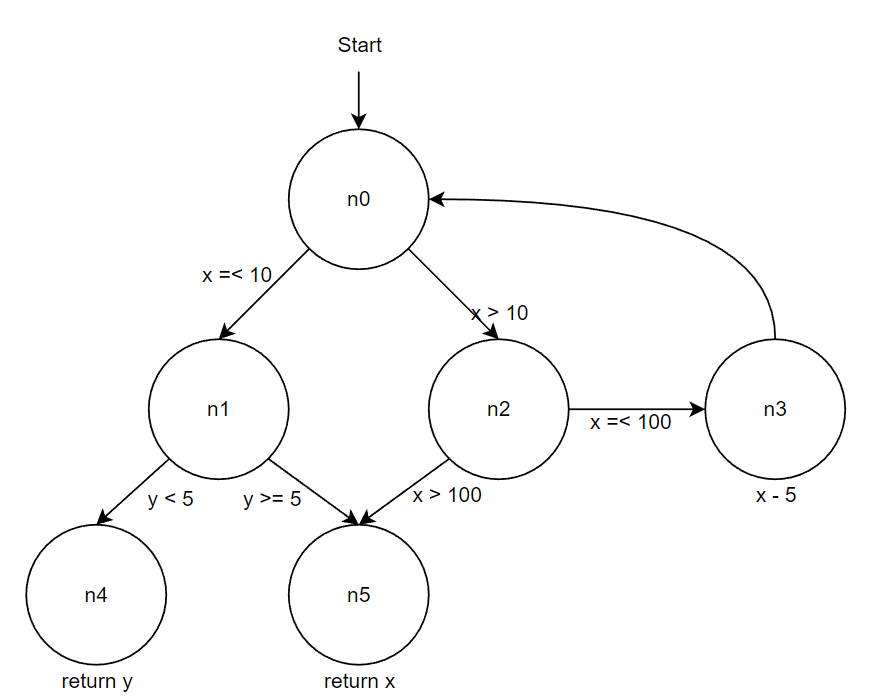
\includegraphics[width=\textwidth,height=\textheight,keepaspectratio]{img/cfg}
    \end{center}
\end{minipage}

Der Code der Funktion $example$ sei nun zu testen.
Mithilfe der zuvor definierten Coveragekriterien können wir Pfade nun Pfade ermitteln und aus diesen Pfaden tests generieren.
Nehme wir zum Beispiel die Node-Coverage.
So müssen wir Pfade finden, sodass jeder Knoten mindestens einmal in einem Test vorkommt.
Mit NodeCoverage sind die Pfade $(N_0, N_2, N_3, N_1, N_5)$ und $(N_0, N_1, N_4)$ ausreichend.
Jeder Knoten wird durch einen Pfad repräsentiert.
Erreicht werden können diese Pfade durch die Variablenauswahl x = 15, y = 10 für Pfad 1 und x = 5, y = 10 für Pfad 2.
Somit haben wir die Tests example(15,10) und example(5,10) welche NodeCoverage erfüllen.
Wir sehen auf anhieb, dass die Node-Coverage nicht ausreichend ist um Code gut zu testen.
Es ist wünschenswert, dass jede Zeile Code im Testprozess mindestens einmal ausgeführt wird (Quelle TODO).
Wir sehen aber, dass z.B. Zeile 4 nie ausgeführt wird durch unsere Tests.
Da die Tests jedoch die Node-Coverage erfüllen müssen wir schlussfolgern, dass die Node-Coverage nicht ausreichend ist.
Somit muss ein stärkeres Coverage-Kriterium her um Code ideal zu testen.
Der interessierte Leser sei an dieser Stelle an \textit{Introduction to Software Testing Kapitel 2.3.1} \cite{software-testing} verwiesen.
Wir wollten hier lediglich zeigen, dass Überdeckungskriterien speziell für den Anwendungsfall auszuwählen sind.
